% ======================================================================
%  Simulation results subsection (paste into Section V).
%  All numbers are produced by the accompanying code (sim/) over the real
%  InTAS Ingolstadt SUMO trace, averaged over 3 random seeds.
% ======================================================================

\subsection{Simulation Results}
\label{subsec:simulation_results}

Fig.~\ref{fig:map_propagation} visualizes encoder propagation over the real
Ingolstadt road network. With road-topology and traffic awareness, the proposed
framework forwards and caches modality-specific encoders along high-traffic
segments where future V2V contacts are likely, so strong encoders reach more
vehicles---including those far from the strong-encoder owners (blue stars). In
contrast, the road/traffic-agnostic scheme leaves many vehicles with low-quality
models (red markers), yielding a lower mean accuracy ($0.63$ vs.\ $0.57$ at the
plotted round).

Fig.~\ref{fig:accuracy} shows the mean model accuracy versus the global round.
The proposed framework consistently outperforms all baselines throughout
training and attains a final accuracy of $0.687$, compared with $0.634$ for
Caching-assisted, $0.635$ for V2V-aware, and $0.636$ for Learning-aware---an
improvement of about $5.1$ percentage points ($8.1\%$ relative) over the best
baseline. The gap widens as training proceeds, indicating faster convergence:
the proposed scheme reaches the baselines' final accuracy roughly $30$ rounds
earlier. Notably, the naive LRU-based Caching-assisted scheme performs on par
with the no-caching baselines, confirming that caching alone is not beneficial
under scarce V2V contact durations; the gain stems from \emph{demand- and
mobility-aware} caching and forwarding.

Fig.~\ref{fig:poor_accuracy} reports the accuracy of poor-data vehicles, i.e.,
those whose local sensing quality is low and that therefore depend most on
receiving strong encoders from others. The proposed framework raises their
accuracy to $0.660$, versus $0.59$--$0.60$ for the baselines, showing that
future-contact-aware encoder propagation effectively serves vehicles with
heterogeneous demand beyond direct V2V encounters.

Fig.~\ref{fig:queue} plots the average virtual-queue backlog $\bar{Q}(k)$.
The proposed scheme maintains the lowest backlog, confirming that the
Lyapunov-guided selection prioritizes persistently unsatisfied learning needs
and keeps the queues stable while maximizing the forwarding utility.

\begin{table}[t]
\centering
\caption{Final performance over the InTAS Ingolstadt trace (mean of 3 seeds).}
\label{tab:final_results}
\begin{tabular}{lccc}
\hline
Scheme & Mean acc. & Poor-data acc. & Final loss \\
\hline
\textbf{Proposed}        & \textbf{0.687} & \textbf{0.660} & \textbf{0.175} \\
Caching-assisted (LRU)   & 0.634 & 0.599 & 0.224 \\
V2V-aware                & 0.635 & 0.601 & 0.211 \\
Learning-aware           & 0.636 & 0.603 & 0.211 \\
\hline
\end{tabular}
\end{table}

\begin{figure}[t]
\centering
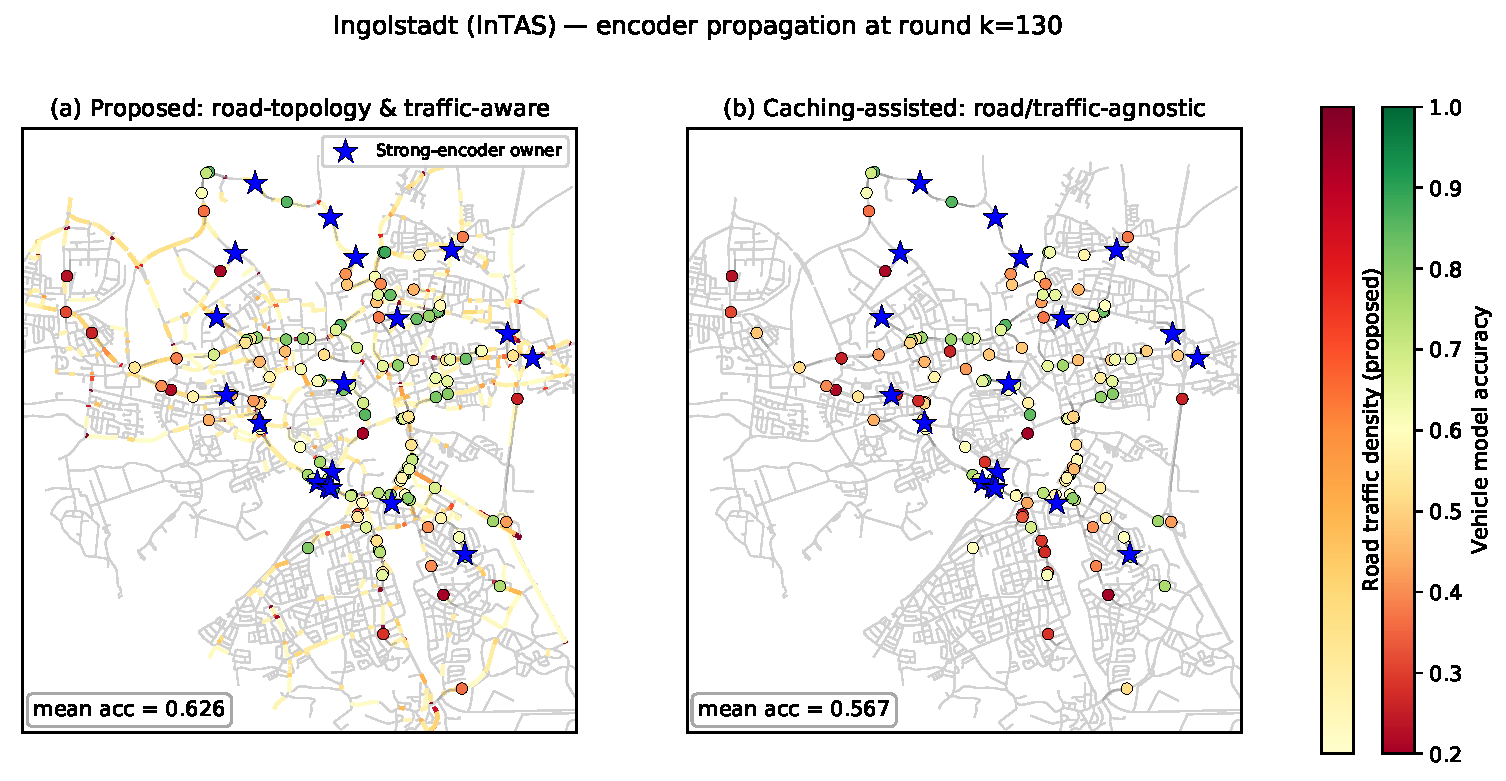
\includegraphics[width=\columnwidth]{Figures/fig_map_propagation.pdf}
\caption{Encoder propagation on the real Ingolstadt (InTAS) map with vehicle
mobility. (a) The proposed road-topology \& traffic-aware scheme (roads colored
by traffic density) propagates strong encoders to more vehicles; (b) the
road/traffic-agnostic scheme leaves more vehicles under-served. Blue stars are
strong-encoder owners; markers are vehicles colored by model accuracy.}
\label{fig:map_propagation}
\end{figure}

\begin{figure}[t]
\centering
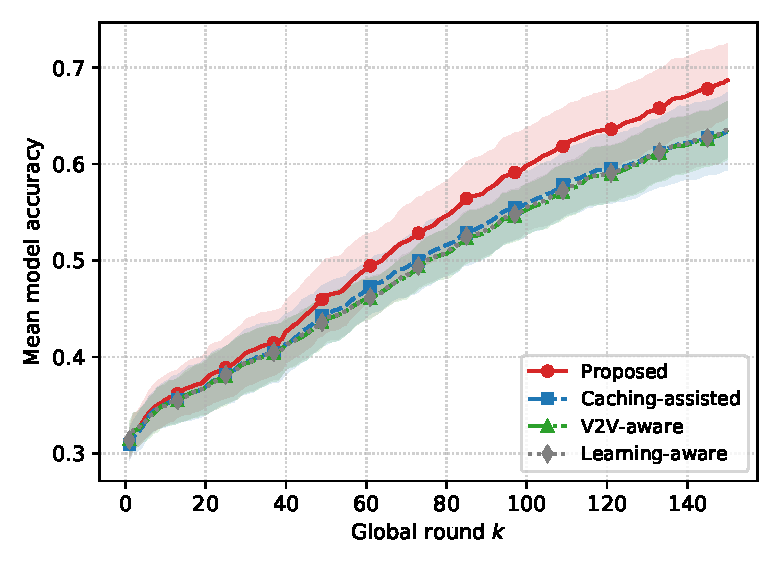
\includegraphics[width=\columnwidth]{Figures/fig_accuracy.pdf}
\caption{Mean model accuracy versus global round (shaded: $\pm$std over seeds).}
\label{fig:accuracy}
\end{figure}

\begin{figure}[t]
\centering
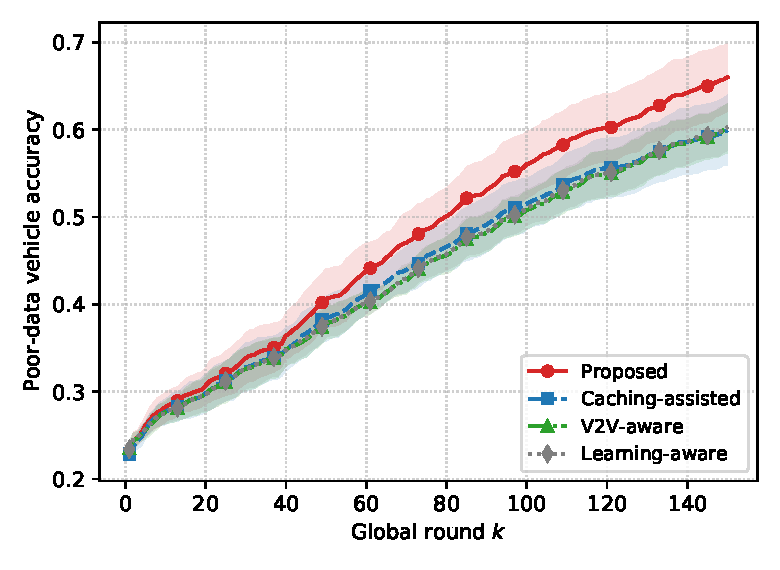
\includegraphics[width=\columnwidth]{Figures/fig_poor_accuracy.pdf}
\caption{Accuracy of poor-data vehicles (heterogeneous modality demand).}
\label{fig:poor_accuracy}
\end{figure}

\begin{figure}[t]
\centering
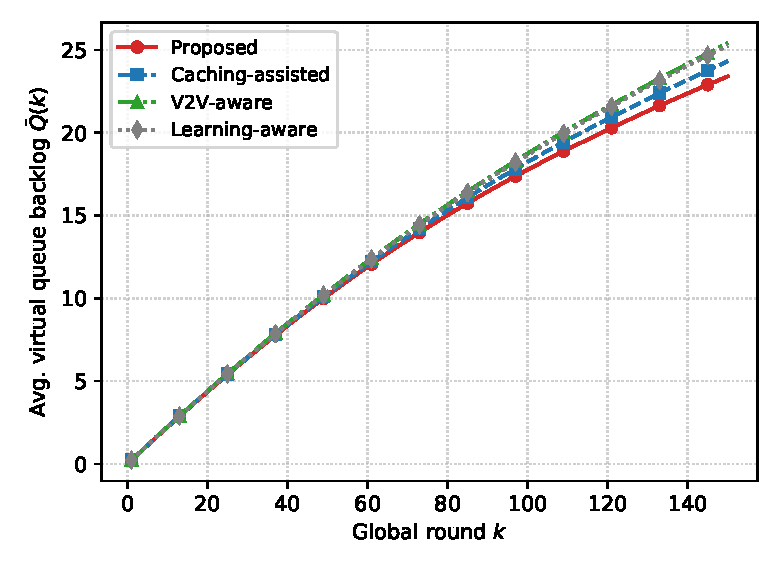
\includegraphics[width=\columnwidth]{Figures/fig_queue.pdf}
\caption{Average virtual-queue backlog $\bar{Q}(k)$ (Lyapunov stability).}
\label{fig:queue}
\end{figure}
